
\section{Задание}

 Дана система из груза массой $m$, связанного с невесомой, жесткой, угруго закрепленной балкой длины $2L$. Один конец балки закреплен на шарнире, расположенном на неподвижной опоре. Балка опирается на пружину, жесткость которой равна $c_0$. В начальный момент времени $t=0$ происходит вертикальный удар по грузу с величиной мгновенного импульса $S$. Если $x$ -- угол отклонения системы от положения равновесия, то система разрушается при $x = \frac{S}{\sqrt{c_0 m L}}$ 

 \begin{figure}[htb]
  \centering
   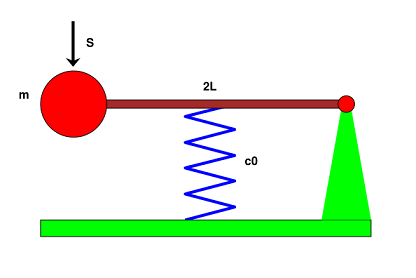
\includegraphics{fig1.png}
 \end{figure}
